\chapter{Preliminaries and Subproblems}
\label{chap:location_nodes}

\section{Path Selection of Mobile elements}
It is known that controlled MULEs can increase a WSN's lifetime by saving energy. But the problem of planning an optimal path and job schedule is a hard problem in general, known as the Data MULE scheduling problem \cite{dms}. It has three components:
\begin{enumerate}
\item Path selection: which trajectory the data mule follows,
\item Speed control: how the data mule changes the speed while moving along the path,
\item and Job scheduling: from which sensor the data mule collects data at each time point.
\end{enumerate}
In this thesis we will focus only on Path selection of the MULEs.

\section{Geometric Disc Covering and Location Nodes}

In the interest of collecting data from sensors in one hop, we propose to cover the sensor field with circular discs of radius equal to the range of the sensors. The centers of these discs are going to be locations where MULEs will pause to collect data from the sensors. We call these positions \emph{location nodes} for convinience. Our path selection heuristic uses location nodes as vertices of a graph embedded on the 2D plane. Ofcourse, we are approximating the communicable region of a sensor to a circular disc, and also assuming that the range of the MULE is greater than that of any sensor (we assume all the sensors are identical in communication range). The centres of these discs are called \emph{location nodes}.

There are many \cite{} \cite{} geometric disc covering heuristics and PTASs, any one of which can be used here. But since PTAS's having high running time \cite{} and hard to implement, we used heuristics for the implementation. Following are some heuristics that we tested on sample fields.

\subsection{Preliminaries}

Let $P$ be the set of points to be covered with discs of radius $R$, in the square field $F$. For any two $p_1, p_2 \in P$, there are two $c_1,c_2 \in F$ (called "crosses" for convinience) such that $p_1$ and $p_2$ will lie at the boundary of a disc of radius $R$ placed at either $c_1$ or $c_2$. We consider points $p_1$ and $p_2$ as covered (barely) by any of the two discs above. For any two points $p_1$ and $p_2$ such that distance between $p_1$ and $p_2$ is less than $2R$, there exist two crosses $c_1$ and $c_2$ ($c_1$ and $c_2$ are said to "involve" $p_1$ and $p_2$ for convinience). Let $C$ be the set of all possible crosses in the field $F$.

A set $S$ of disc centres such that they cover all the points in the field $F$ is called a solution of the MGDC problem in the field $F$. Let $S_1$ be such a solution. Then there exists a solution $S_2 \subset C$ such that $|S_1|=|S_2|$.

\subsection{Heuristics}

\begin{description}

\item[JGRD] This is originally a set cover heuristic \cite{jgreedy}. Consider the set $P$ as the target set to be achieved from the union of smaller subsets, and the discs centered at the crosses in $C$ represent the subsets of points covered by them. Our problem of MGDC then becomes a set cover problem. \cite{jgreedy} gives a greedy heuristic for this.

\item[GRD] (We are not aware of any other work using this heuristic) Let the list of all sensor positions in the field $F$ be $L$. First sort $L$ according to their (x,y) position co-ordinates (first by x co-ordinate and then by y co-ordinate). Starting from the first sensor $p$ in the list, pick the disc which covers maximum number of uncovered sensors and covers $p$ too. To do this, compute all the crosses in $C$ which involve $p$. Place a disc of radius $R$ at each of the crosses, and choose the cross whose disc covers the most number of points. Choose the next uncovered sensor in $L$ and repeat the covering procedure, until all sensors are covered.

\item[SHFT] The shifting strategy from \cite{shifting}.
\item[SEL] For any sensor $s$, let $L$ be the set of discs covering it. Pick the disc which covers the least number of sensors.
\item[RND] Randomly pick discs until all the sensors are covered. Just for sake of comparision with other heuristics.
\end{description}

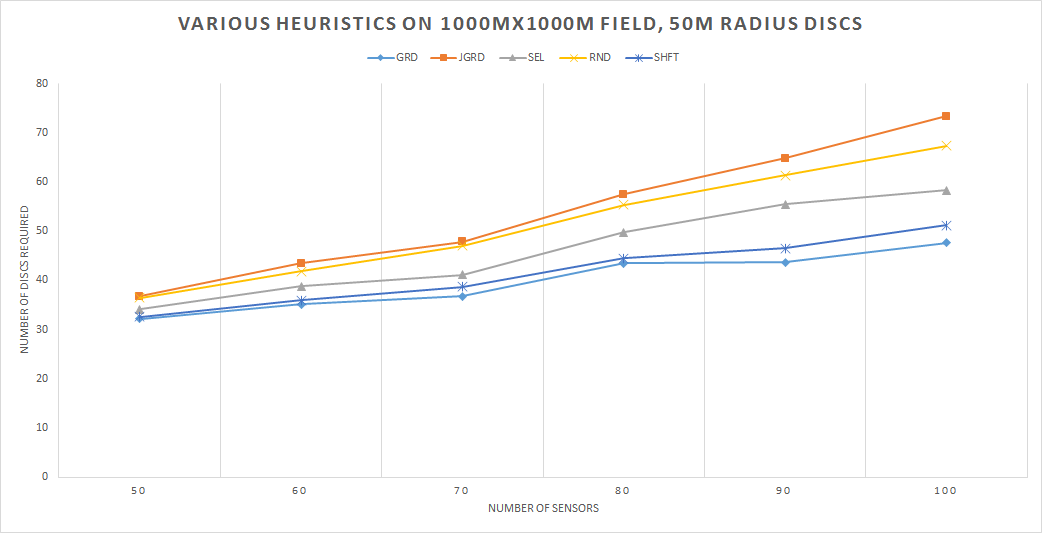
\includegraphics[width=15cm]{discs}